%File: cogni_map_workshop.tex
\documentclass[letterpaper]{article}
\usepackage{aaai2026}
\usepackage{times}
\usepackage{helvet}
\usepackage{courier}
\usepackage[hyphens]{url}
\usepackage{graphicx}
\urlstyle{rm}
\def\UrlFont{\rm}
\usepackage{natbib}
\usepackage{caption}
\usepackage{amsmath}
\usepackage{amssymb}
\frenchspacing
\setlength{\pdfpagewidth}{8.5in}
\setlength{\pdfpageheight}{11in}

\pdfinfo{
/TemplateVersion (2026.1)
}

\setcounter{secnumdepth}{0}

\title{Cogni Map: Real-Time Detection of Cognitive Actions in Language Models Through Linear Probing}

\author{
    Ivan Chulo, Ananya Joshi
}
\affiliations{
    Johns Hopkins University\\
    Baltimore, MD 21218 USA\\
}

\begin{document}

\maketitle

\begin{abstract}
Understanding cognitive processes in large language models remains challenging, as we lack systematic tools to track internal reasoning patterns during text generation. To address this disconnect, we developed Cogni Map—a mechanistic interpretability tool leveraging linear probes to detect 45 cognitive actions spanning metacognitive, analytical, creative, and emotional categories. Binary one-vs-rest probes were trained on internal activations from 30 layers of Gemma-3-4B using 31,500 synthetic examples with augmented prompting for consistent extraction. Our approach achieved 0.78 average AUC-ROC across all cognitive actions, with layer 9 reaching peak performance (0.948 AUC). Additionally, regression-based sentiment probes trained on 1,400 examples achieved R²=0.851, revealing that emotional valence is encoded in early layers (1-11) while cognitive abstractions require mid-layer processing (5-24). This distinct layer specialization suggests a hierarchical processing architecture where surface-level sentiment precedes higher-level cognition. Application to therapy transcripts revealed therapist-dominant actions (\textit{perspective\_taking}, \textit{accepting}) versus client-dominant patterns (\textit{reconsidering}, \textit{self\_questioning}), aligning with person-centered therapy principles. Cogni Map bridges mechanistic interpretability and cognitive science, offering both quantitative probe analysis and qualitative exploration through an interactive terminal interface for understanding AI reasoning in diverse applications.
\end{abstract}

\section{Introduction}

Understanding the internal reasoning of large language models (LLMs) is crucial for ensuring their safety, interpretability, and alignment \cite{bereska2024mechanistic}. While previous studies have focused on profiling user attributes from conversations \cite{chen2024designing}, less attention has been given to identifying the \textit{cognitive actions} exhibited by the model during text generation.

This project introduces Cogni Map, a mechanistic interpretability tool designed to explore and annotate 45 cognitive actions spanning metacognitive, analytical, creative, and emotional categories. These actions, inspired by taxonomies from cognitive psychology, offer a detailed vocabulary for describing an AI's "thought processes," from \textit{pattern\_recognition} and \textit{hypothesis\_generation} to \textit{emotional\_reappraisal}. Cogni Map supports both quantitative analysis of cognitive patterns and qualitative exploration via an interactive TUI. The methodology is built upon linear probing techniques \cite{alain2016understanding} to extract representations of cognitive actions from transformer activations, enabling researchers to observe the cognitive functions that are active during generation.

\textbf{Contributions:} (1) A synthetic dataset of 31,500 examples spanning 45 cognitive actions and sentiment valence; (2) Binary cognitive action probes and regression-based sentiment probes trained across 30 layers of Gemma-3-4B, achieving 0.78 AUC-ROC and 0.851 R² respectively, revealing distinct layer specialization patterns (sentiment in early layers 1-11, cognition in mid-layers 5-24); (3) A toolkit for quantitative and qualitative analysis including an interactive terminal interface; (4) Practical application to therapy transcript analysis demonstrating role-specific cognitive patterns.

\section{Methodology}

\textbf{Cognitive Action Taxonomy.} A taxonomy of 45 cognitive actions was defined, organized into four categories: \textit{Metacognitive} (13 actions, e.g., \textit{reconsidering}, \textit{updating\_beliefs}), \textit{Analytical} (12 actions, e.g., \textit{analyzing}, \textit{evaluating}), \textit{Creative} (6 actions, e.g., \textit{divergent\_thinking}, \textit{reframing}), and \textit{Emotional} (14 actions, e.g., \textit{emotional\_reappraisal}).

\textbf{Activation Capture and Probing.} Following established probing methodologies \cite{alain2016understanding,chen2024designing}, activations were extracted from 30 of the 34 layers of Gemma-3-4B using nnsight. During both activation capture and inference, inputs were augmented with task-specific suffixes ("The cognitive action being demonstrated here is" for cognitive probes; "The sentiment of this section is" for sentiment probes) to ensure consistent extraction from the final token representation. A \textbf{one-vs-rest} strategy was used to train 45 independent binary linear probes, which allows for per-action interpretability and the flexibility to mix optimal layers for each action during inference. Training was performed with an AdamW optimizer, cosine annealing scheduler, and early stopping, using an AUC-ROC metric to handle the severe class imbalance.

\textbf{Sentiment Probe Training.} In addition to cognitive action detection, regression-based sentiment probes were trained to capture continuous emotional valence rather than binary classification. Unlike cognitive probes that output binary predictions (0 or 1), sentiment probes use linear regression to produce unbounded continuous scores where negative values indicate negative sentiment and positive values indicate positive sentiment, with magnitude reflecting intensity. Training data consisted of 1,400 synthetic examples (700 positive, 700 negative) generated via vLLM-optimized batch inference with diverse emotional contexts spanning 10 emotions per sentiment category. Probes were trained across all 30 layers using MSE loss with targets normalized to [-1, +1]. The regression approach enables more nuanced sentiment analysis than binary classification, capturing gradations of emotional intensity in generated text.

\textbf{Data Generation.} The training dataset consists of 31,500 synthetic examples generated using Gemma 3 4b. This includes 700 examples for each of the 45 cognitive actions and 1,400 examples for sentiment analysis (700 positive, 700 negative).

\section{Results}

\textbf{Probe Performance.} The binary probes demonstrated strong performance, achieving an average AUC-ROC of 0.78 and an average F1 score of 0.68 across all 45 cognitive actions. Top-performing probes included \textit{suspending\_judgment} (0.988 AUC) and \textit{counterfactual\_reasoning} (0.984 AUC), while more challenging actions included \textit{emotion\_responding} (0.778 AUC). These results confirm that cognitive actions have linearly separable representations within Gemma-3-4B's activation space \cite{alain2016understanding}.

\textbf{Layer Specialization.} A distinct pattern of layer specialization was observed across the 30 analyzed layers. Cognitive action probes achieved peak performance at layer 9 (AUC-ROC: 0.948) with strong performance across mid-layers (5-24), while sentiment probes peaked earlier at layer 7 (R²=0.851) with optimal performance concentrated in layers 1-11 before degrading sharply. This contrasts sharply between cognitive and sentiment representations, suggesting that sentiment is encoded in early layers while higher-level cognitive abstractions require deeper mid-layer processing, revealing a hierarchical architecture where surface-level emotional features precede complex cognitive patterns.

\textbf{Application: Therapy Transcript Analysis.} Cogni Map was applied to analyze a therapy session transcript, comparing the cognitive actions of the therapist and the client. The analysis revealed that therapist-dominant actions included \textit{metacognitive monitoring}, \textit{meta awareness}, and \textit{questioning}. In contrast, client-dominant actions were \textit{analyzing}, \textit{accepting}, and \textit{noticing}. These findings align with the principles of person-centered therapy \cite{rogers1951client}, where the therapist fosters an environment for the client's self-exploration.

\section{Discussion and Future Work}

Cogni Map builds upon prior work in interpretability \cite{alain2016understanding,chen2024designing} but shifts the focus from modeling external users to tracking the internal cognitive processes of the model itself. While Chen et al. demonstrated probing for user demographics, we track cognitive actions in model-generated content—a complementary approach to representation engineering work \cite{zou2023representation}.

\textbf{Hierarchical Processing Architecture.} The divergent layer specialization between sentiment and cognitive probes reveals fundamental insights into transformer information processing. Sentiment's early-layer encoding (layers 1-11, peak at layer 7) suggests it functions as a low-level feature detected from lexical and syntactic patterns, while cognitive actions require deeper semantic processing in mid-layers (5-24, peak at layer 9). This processing hierarchy mirrors cognitive science theories distinguishing affective (emotional) from cognitive processing systems, suggesting that transformer architectures may naturally develop analogous hierarchical representations. The sharp performance degradation for sentiment probes in later layers (negative R² after layer 11) indicates that these early representations are progressively overwritten as the model shifts focus toward next-token prediction, while cognitive abstractions remain accessible deeper in the network.

\textbf{Limitations} of this study include the reliance on synthetic data, the focus on a single model (Gemma-3-4B) and the assumption of independence between cognitive actions.

\textbf{Future directions} include extending the tool to larger models, training on human-annotated data, and exploring applications in downstream tasks like ToM in LLMs and AI alignment as well as other domains like education, mental health, psychology and sociology.

\textbf{Broader Impact:} This tool's real-time cognitive monitoring unlocks several key downstream applications. In education and mental health, it can power adaptive learning tools and responsive AI companions. For AI safety, it enables process-based supervision by flagging harmful reasoning patterns before they generate output. This also enhances human-AI collaboration by creating assistants that dynamically adapt their cognitive approach to a user's task.

\section{Conclusion}

Cogni Map is a practical tool for exploring and annotating 45 cognitive actions and sentiment valence in language models. By using linear probes on the internal activations of Gemma-3-4B, this work successfully identified and analyzed cognitive patterns and emotional valence, revealing specialized layer-dependent representations with distinct hierarchies: sentiment encoded in early layers (1-11) and cognitive abstractions in mid-layers (5-24). The toolkit, which supports both quantitative and qualitative analysis, has demonstrated its utility in real-world applications, bridging the gap between mechanistic interpretability and cognitive science. The full source code, trained probes, and datasets are available on GitHub.

\bibliography{cogni_map_workshop}

\clearpage
\appendix

\section{Additional Visualizations}

\begin{figure*}[t]
\centering
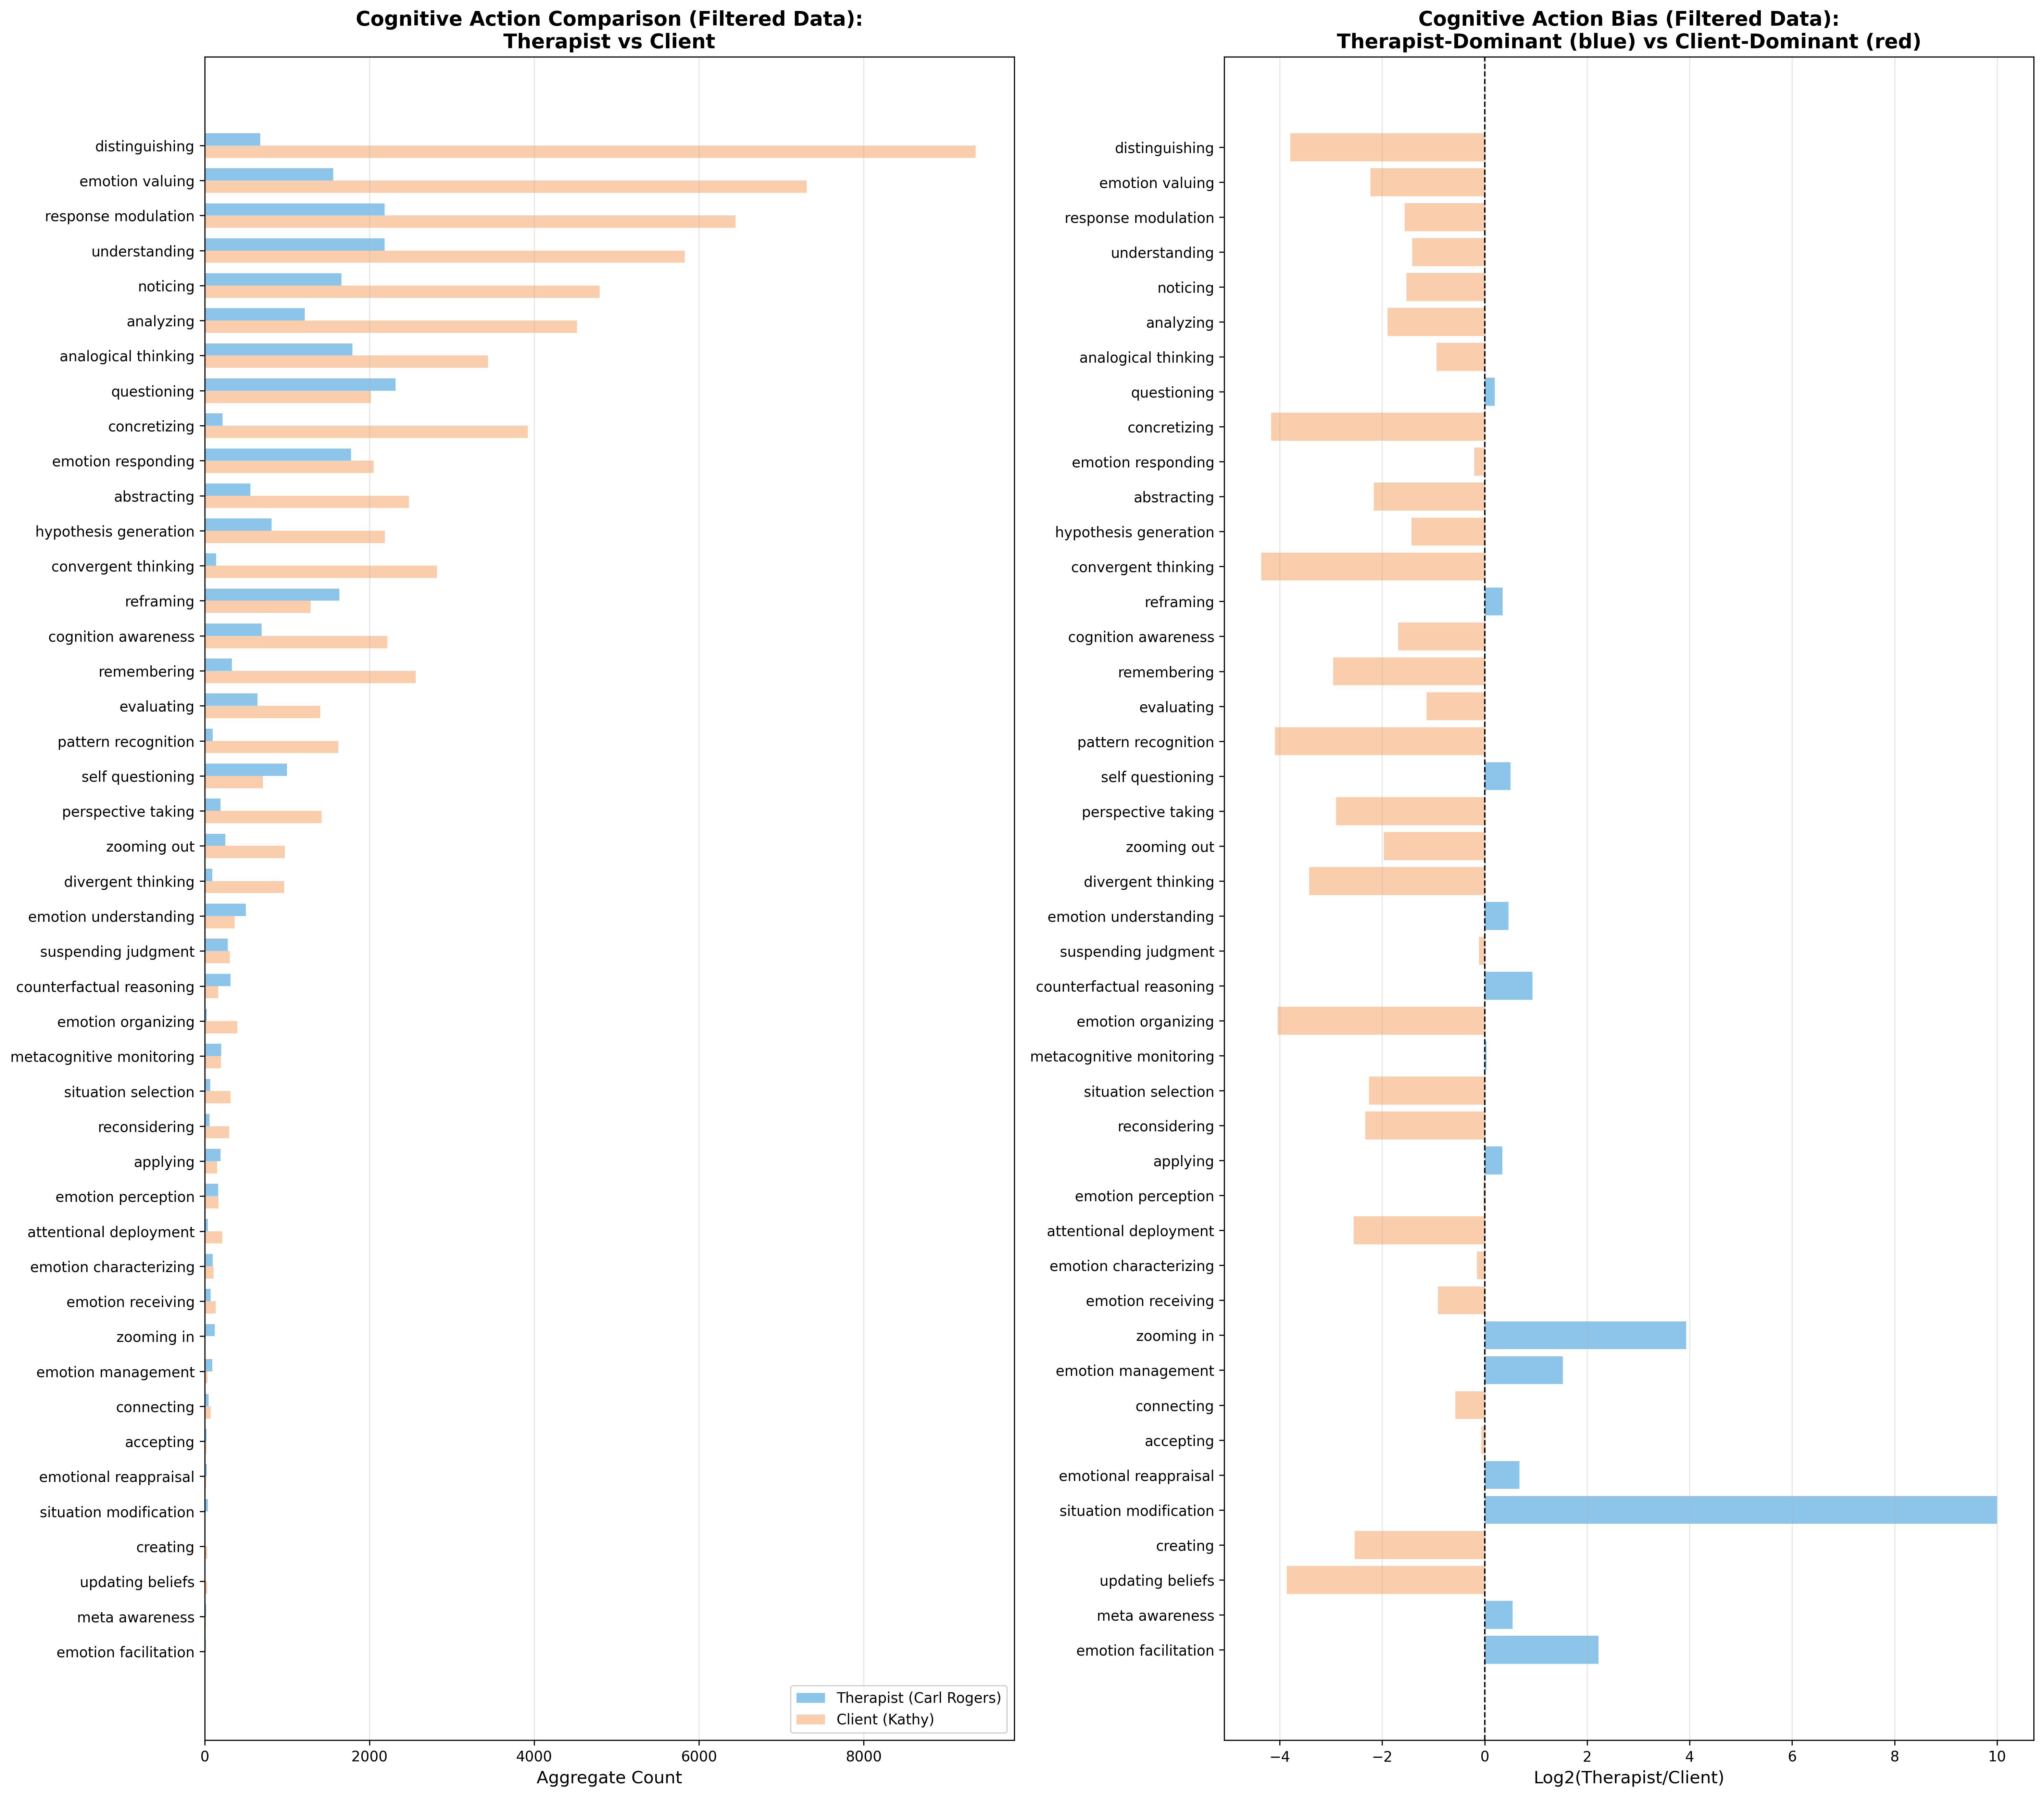
\includegraphics[width=\textwidth]{../Keep_viz/rogers_kathy_comparison.png}
\caption{Therapy session analysis comparing cognitive action patterns between therapist (Carl Rogers) and client (Kathy). Left panel shows aggregate counts of cognitive actions for both participants across filtered data. Right panel displays cognitive action bias as log2 ratio, highlighting therapist-dominant actions (blue) such as \textit{situation\_modification}, \textit{emotional\_reappraisal}, and \textit{emotion\_facilitation}, versus client-dominant actions (red) including \textit{zooming\_in}, \textit{self\_questioning}, and \textit{applying}. These patterns align with person-centered therapy principles.}
\label{fig:therapy_comparison}
\end{figure*}

\begin{figure*}[t]
\centering
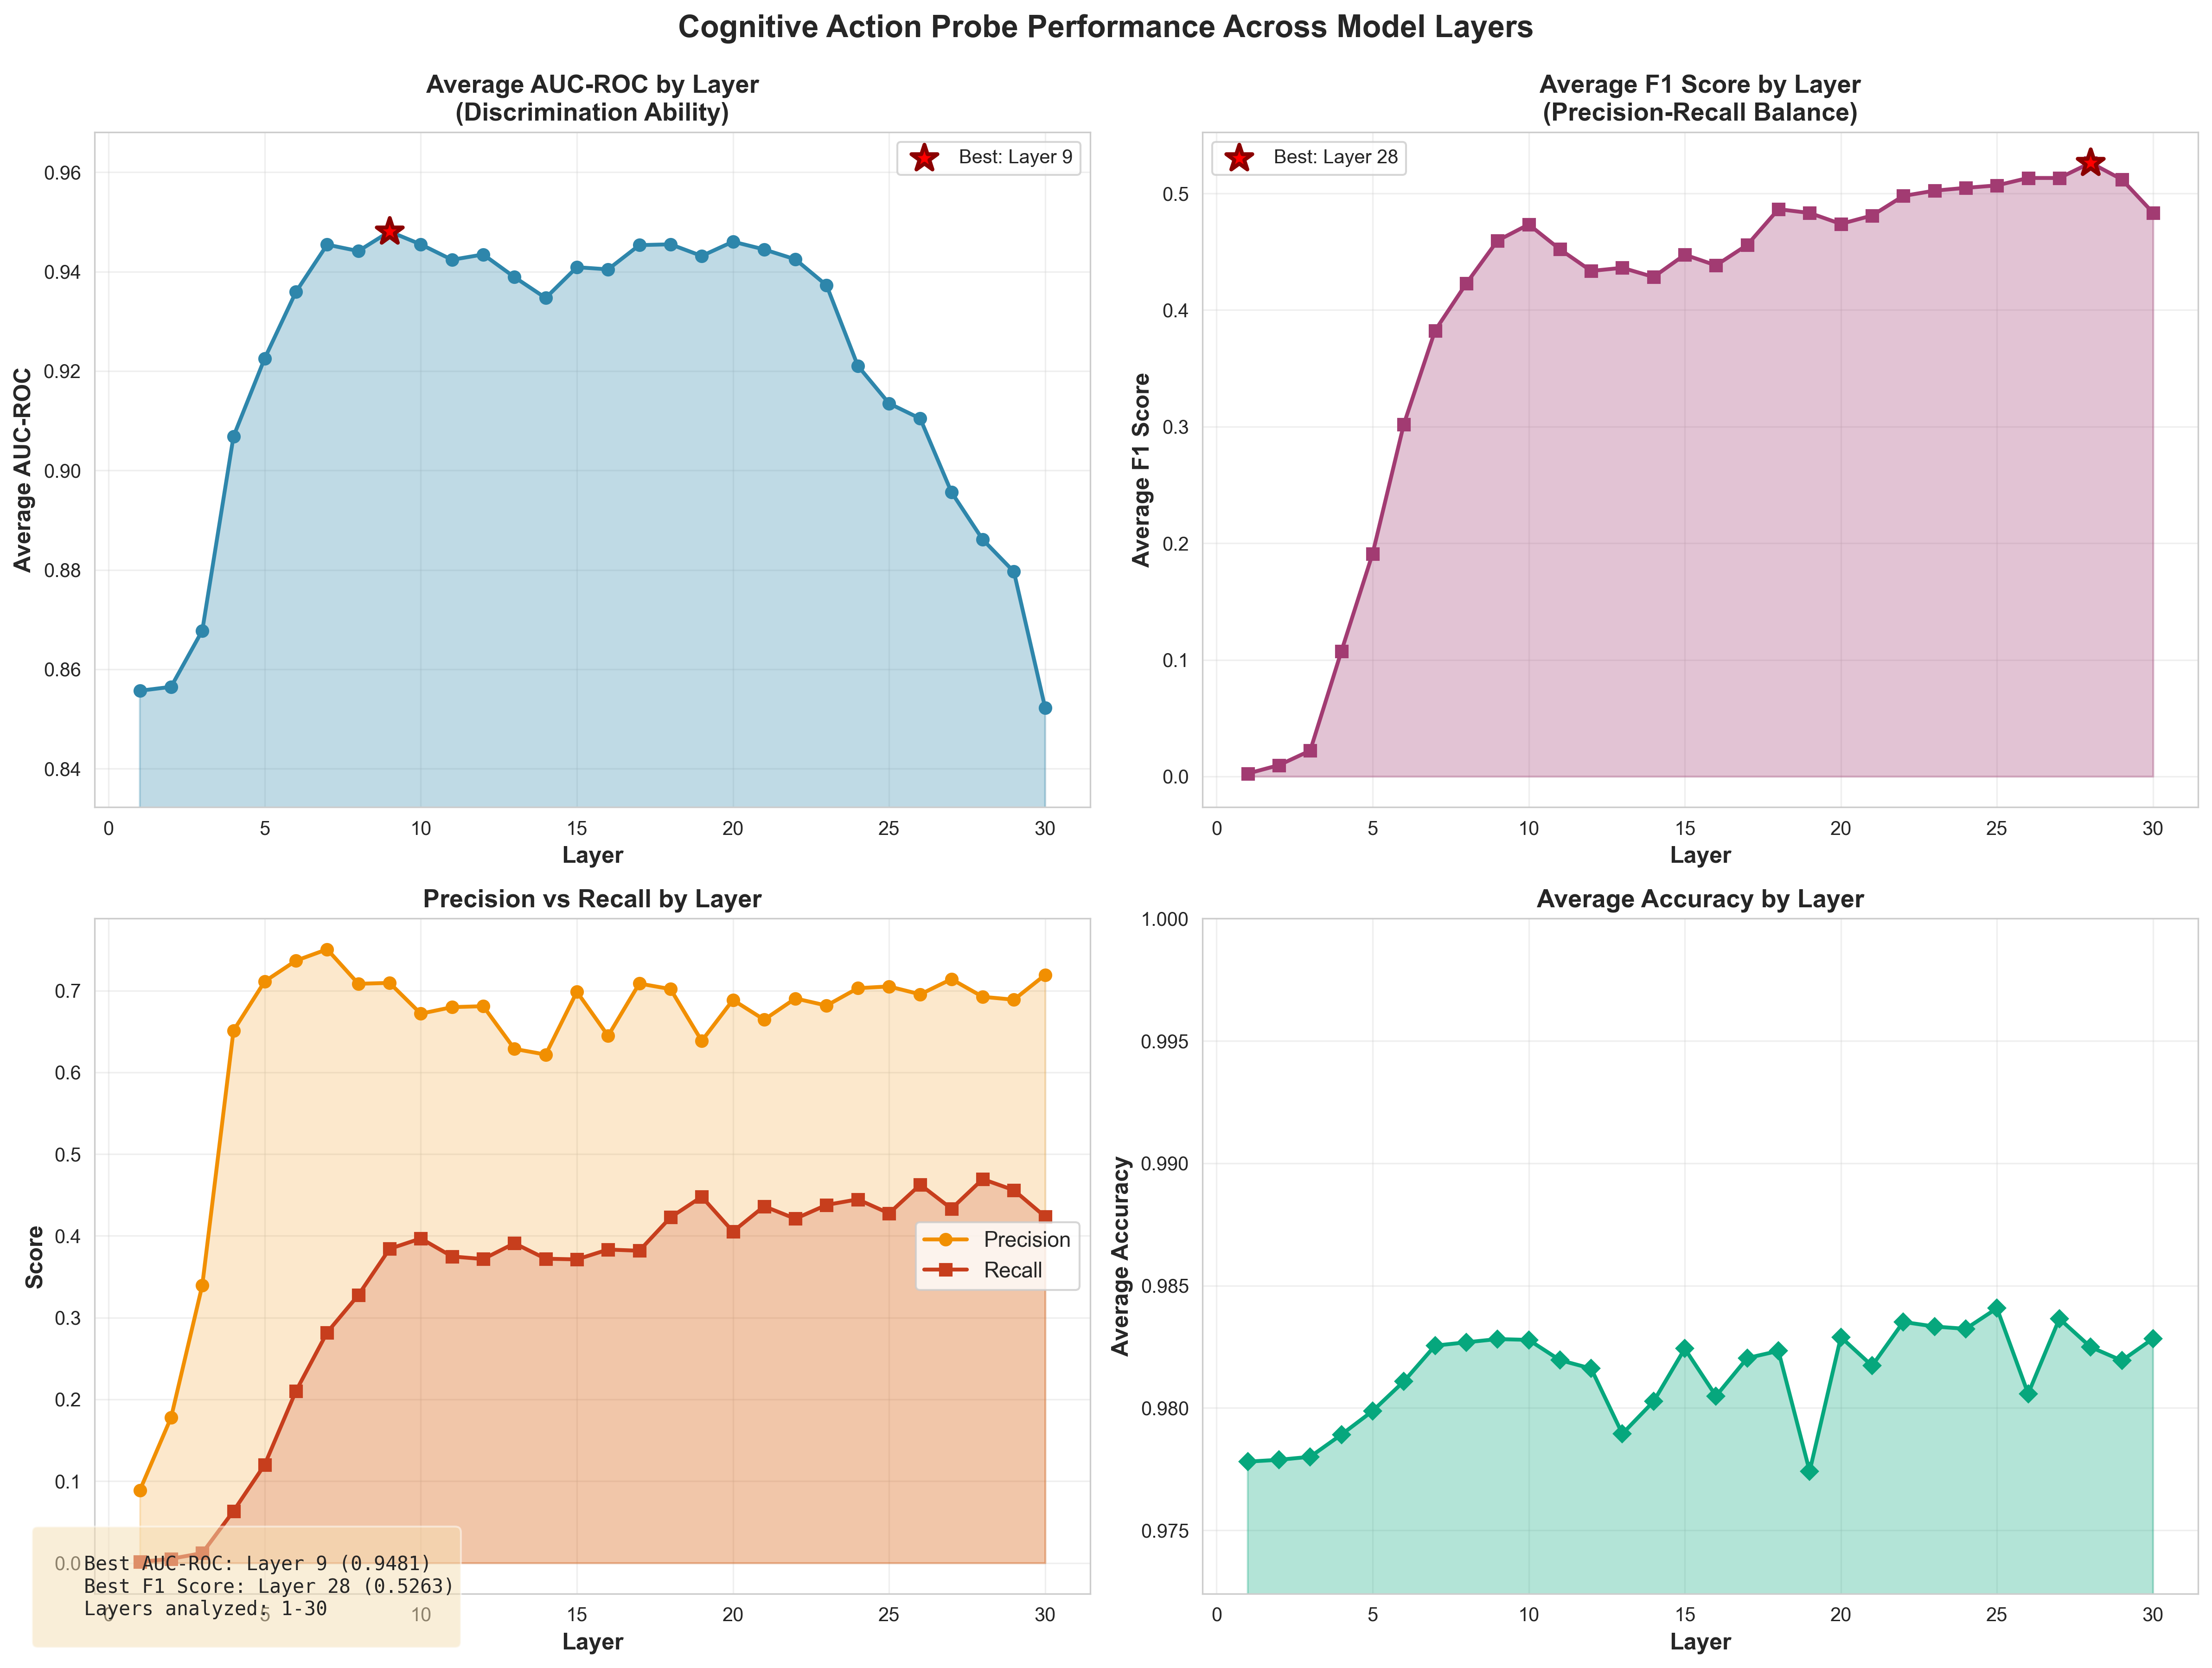
\includegraphics[width=\textwidth]{../data/cognitive_probe_performance_by_layer.png}
\caption{Cognitive action probe performance across all 30 layers of Gemma-3-4B. The visualization shows average AUC-ROC scores for each layer, with Layer 9 achieving peak performance (0.948 AUC-ROC). Strong performance is maintained across mid-layers (5-24), while early and late layers show degraded performance. This pattern suggests that early layers focus on surface-level features, mid-layers capture high-level cognitive abstractions, and late layers optimize for next-token prediction, potentially overwriting intermediate representations.}
\label{fig:layer_performance}
\end{figure*}

\begin{figure*}[t]
\centering
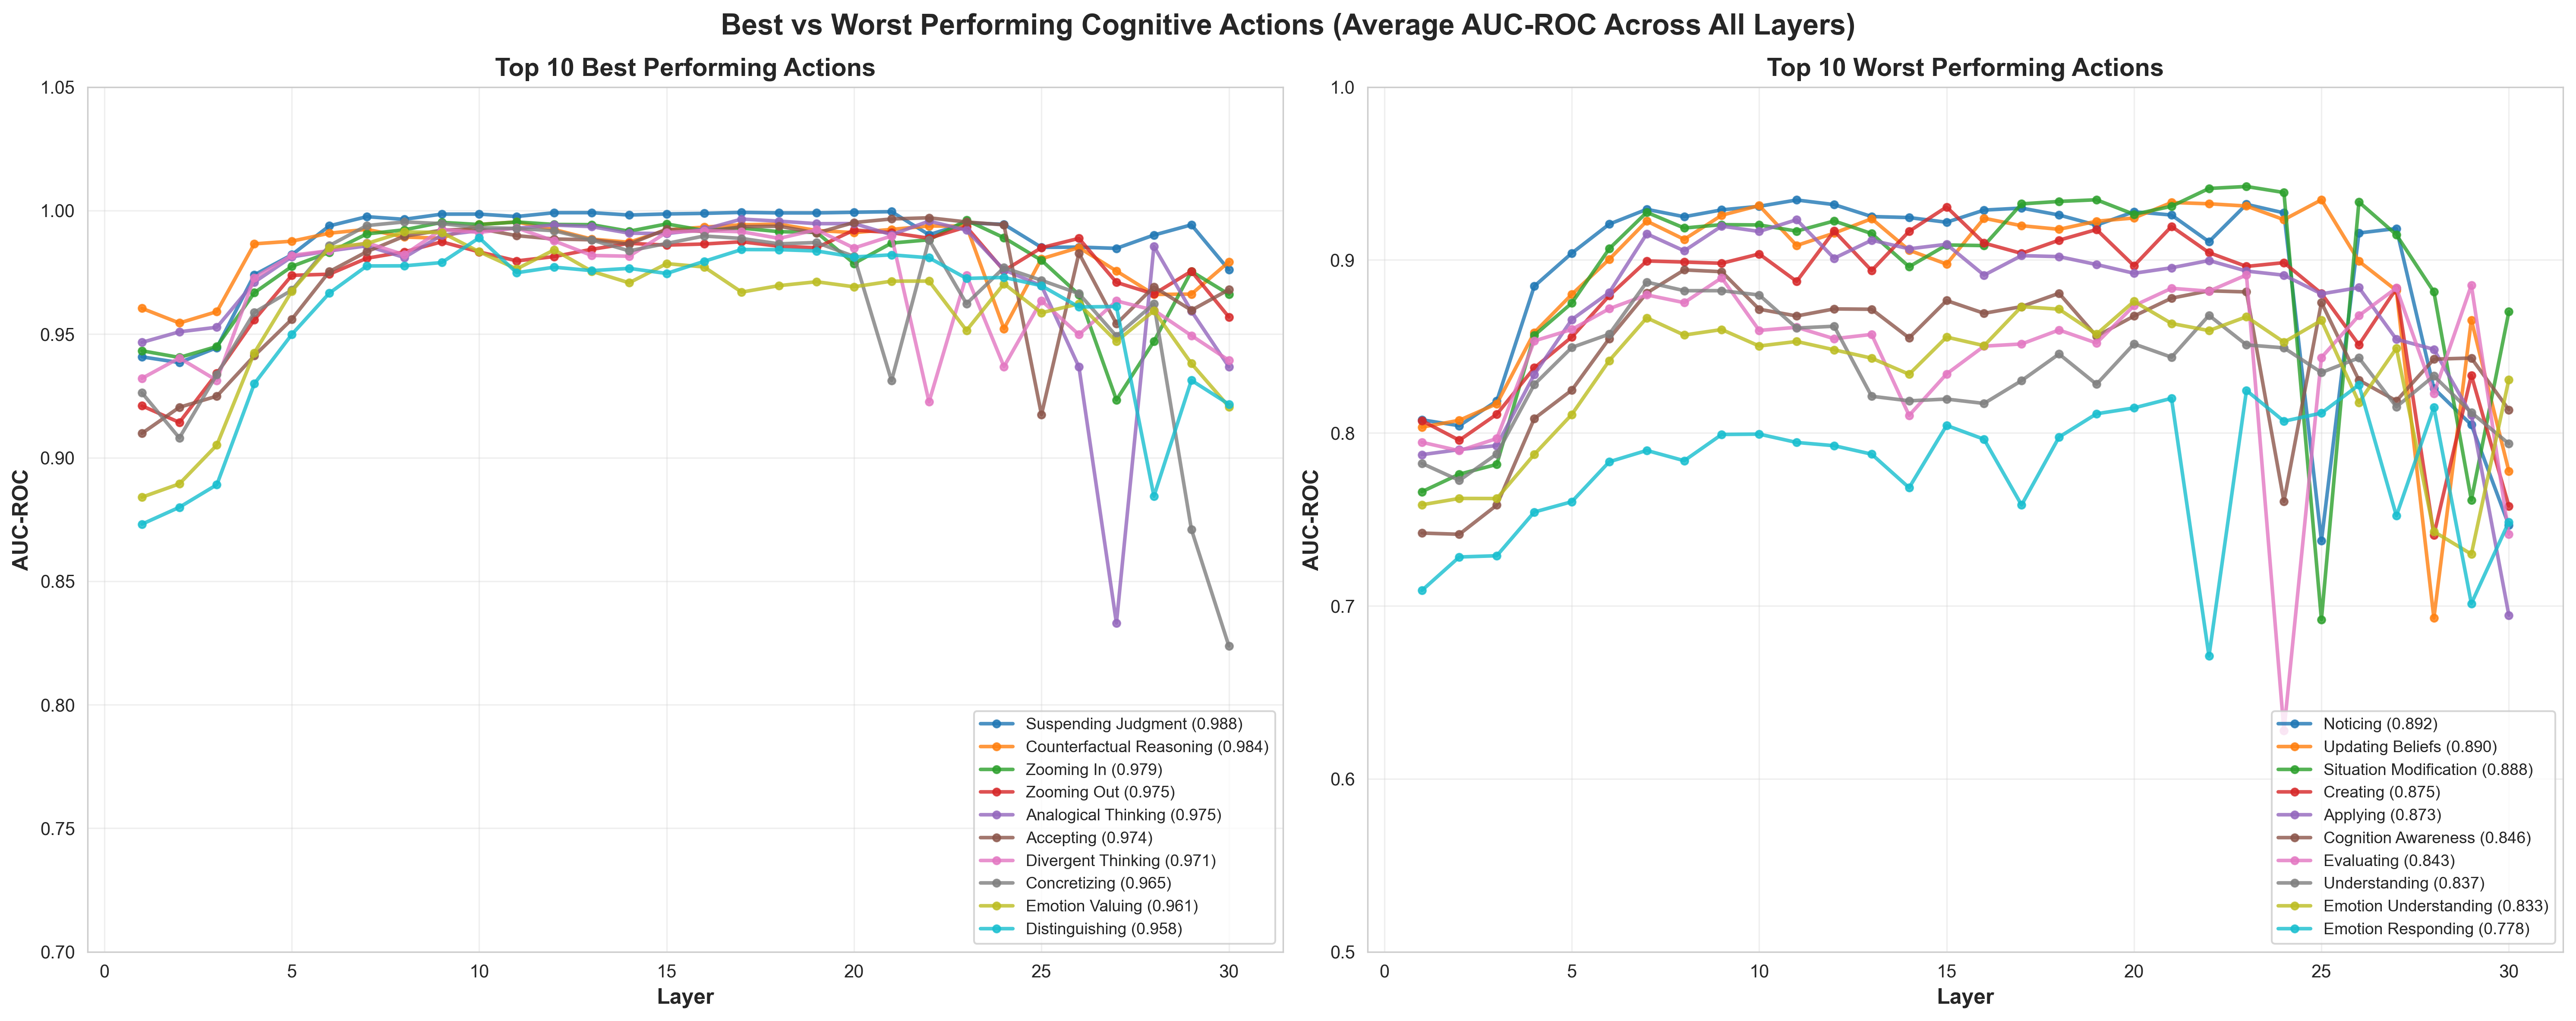
\includegraphics[width=\textwidth]{../data/best_worst_actions.png}
\caption{Comparison of top 10 and bottom 10 performing cognitive actions ranked by average AUC-ROC across all layers. Best performers like \textit{suspending\_judgment} (0.988) and \textit{counterfactual\_reasoning} (0.984) show consistently high performance and distinct activation patterns across most layers. Worst performers like \textit{emotion\_responding} (0.778) and \textit{understanding} (0.837) exhibit more variability and lower overall discrimination ability, suggesting these concepts may be more distributed or context-dependent in the model's representation space.}
\label{fig:best_worst}
\end{figure*}

\begin{figure*}[t]
\centering
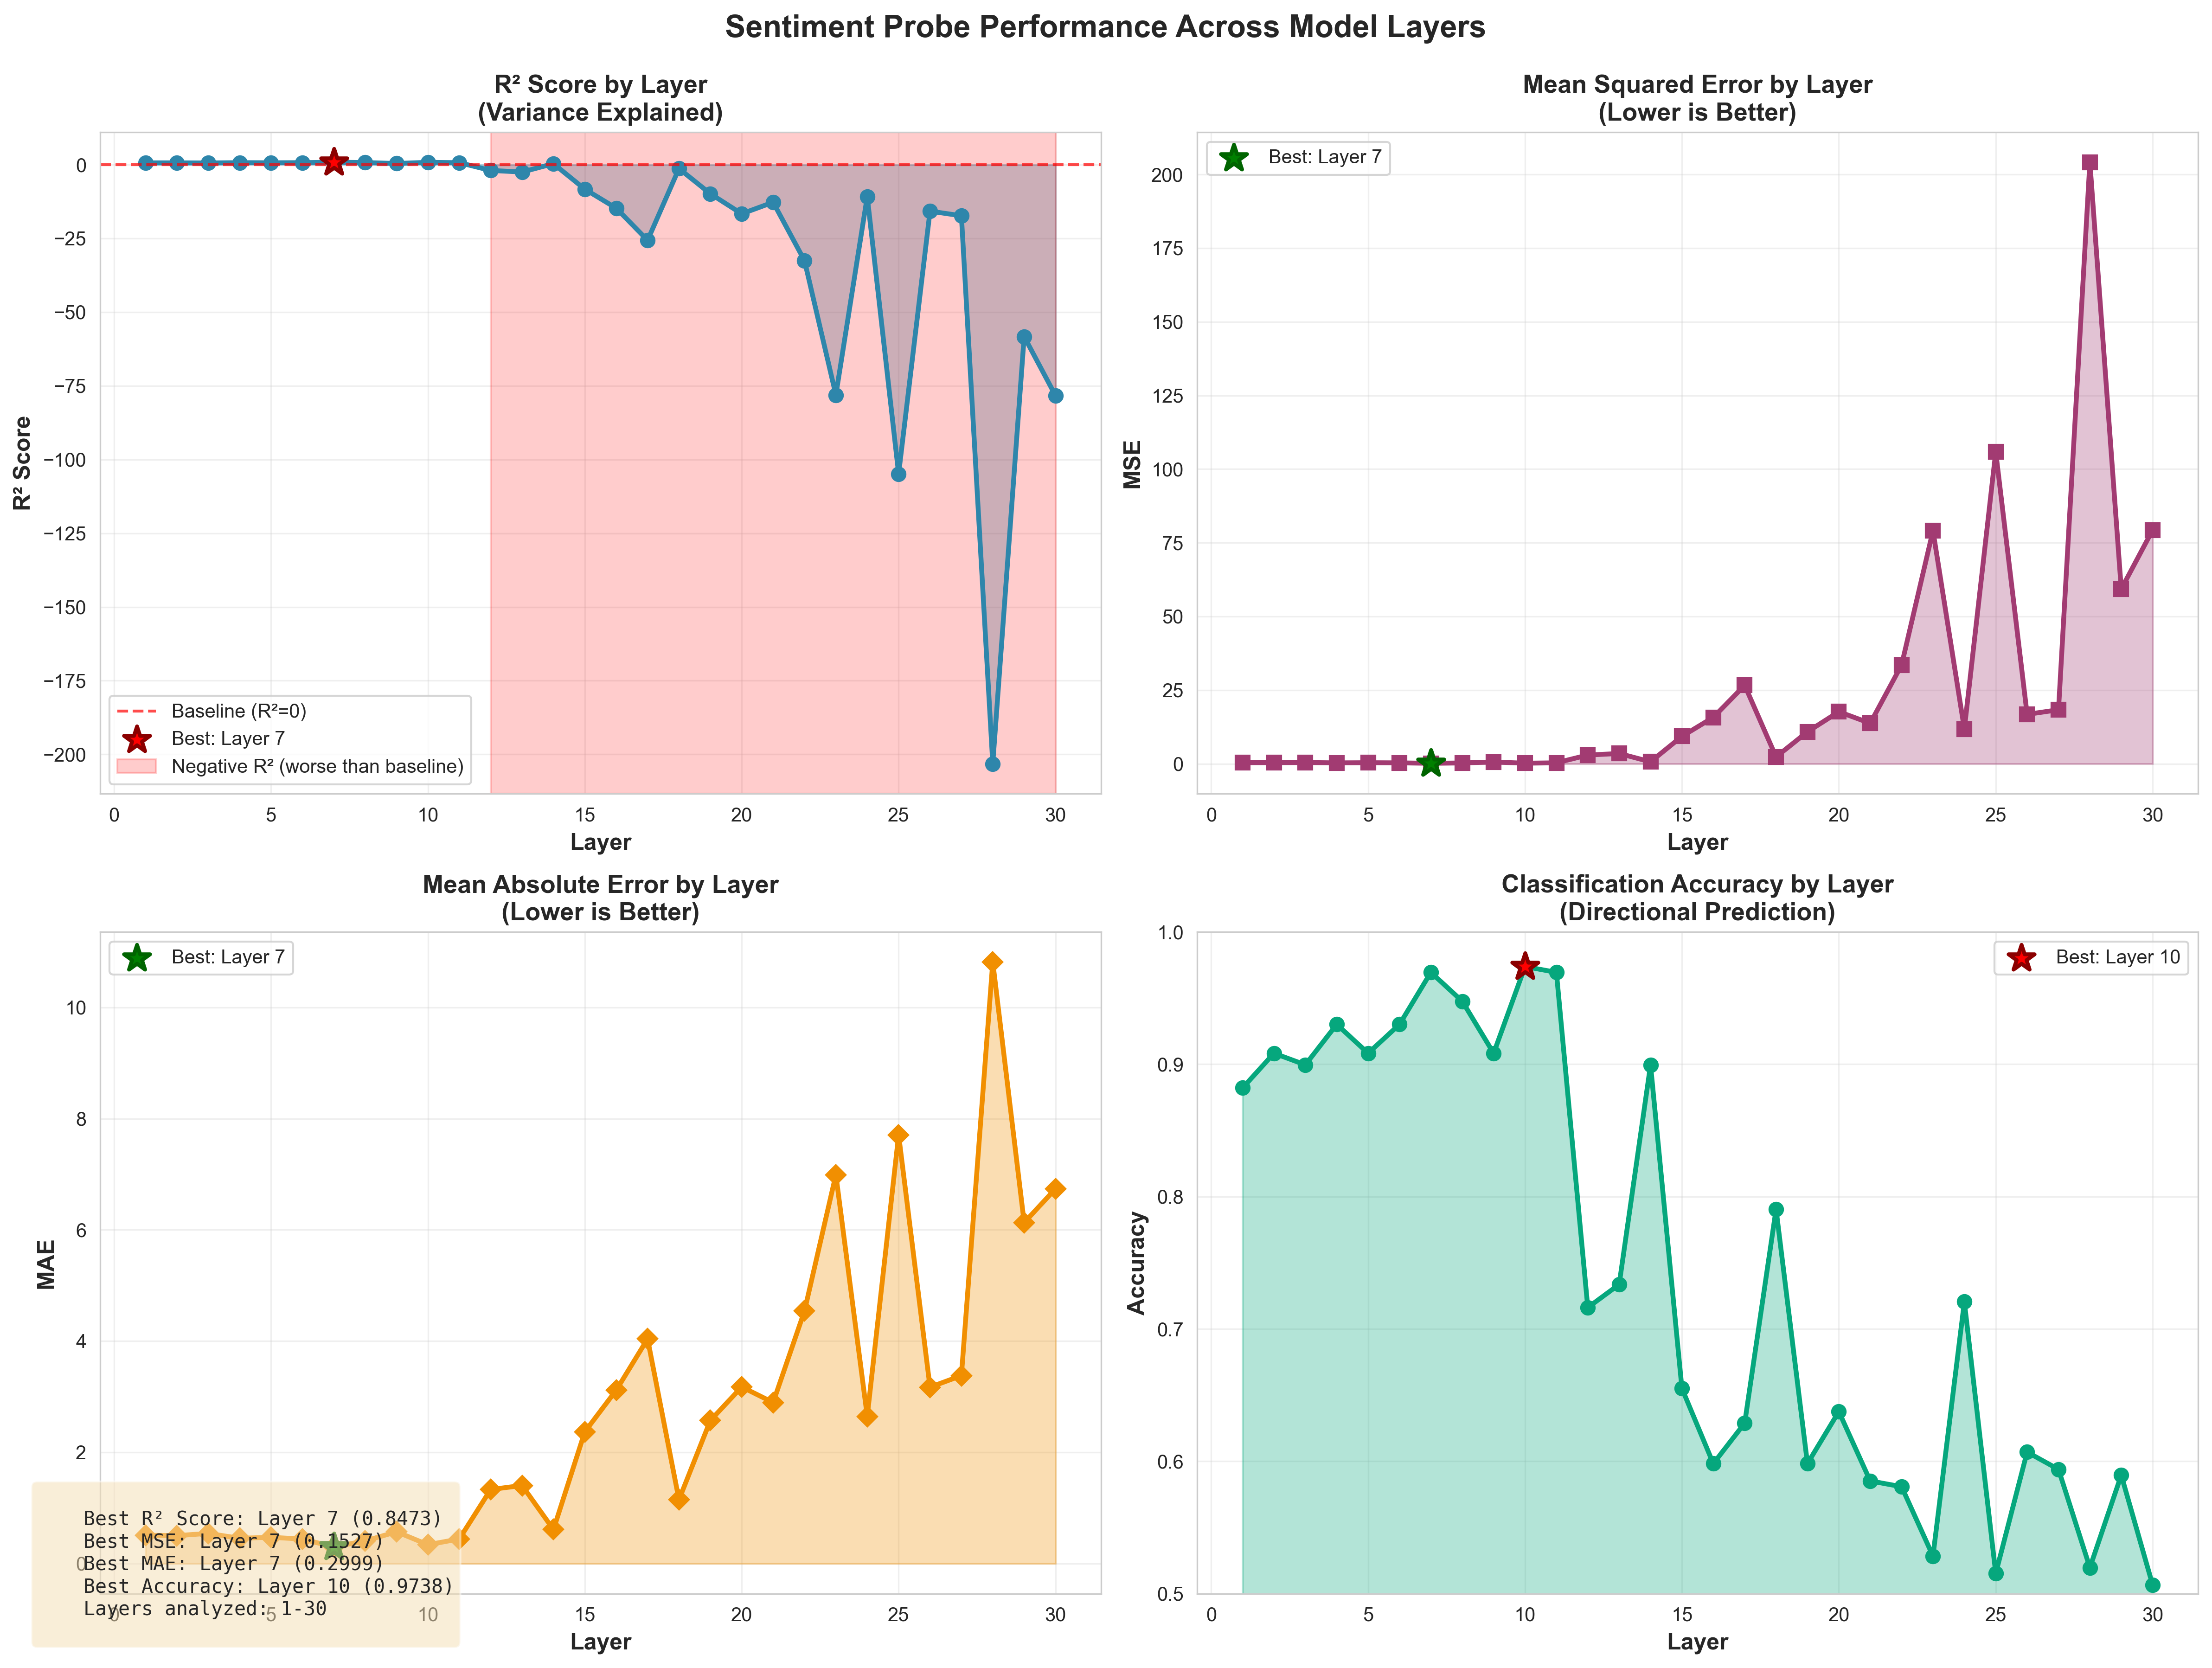
\includegraphics[width=\textwidth]{../data/sentiment_probe_performance.png}
\caption{Sentiment probe performance across all 30 layers showing contrasting specialization pattern compared to cognitive probes. Optimal performance is concentrated in early-to-mid layers (1-11) with Layer 7 achieving peak R²=0.851 (85.1\% variance explained), MSE=0.143, and 96.9\% accuracy. Sharp degradation occurs after Layer 11 with negative R² values in layers 12-30, indicating sentiment representations are encoded earlier in the processing hierarchy than higher-level cognitive abstractions. The four panels show R² Score (top-left), Mean Squared Error (top-right), Mean Absolute Error (bottom-left), and Classification Accuracy (bottom-right).}
\label{fig:sentiment_performance}
\end{figure*}

\end{document}
